%% OptiVision RAG --- IEEE conference paper
%% Compile with pdfLaTeX. Overleaf: upload this file plus figs/ and pick pdfLaTeX.
\documentclass[conference]{IEEEtran}
\IEEEoverridecommandlockouts

\usepackage{cite}
\usepackage{amsmath,amssymb}
\usepackage{graphicx}
%% Look in figs/ first, then the project root, so the paper builds whether the
%% figures were uploaded into a figs/ folder or dropped loose at the top level.
\graphicspath{{figs/}{./}}
\usepackage{booktabs}
\usepackage{multirow}
\usepackage{url}
\usepackage[hidelinks]{hyperref}

\def\BibTeX{{\rm B\kern-.05em{\sc i\kern-.025em b}\kern-.08em
    T\kern-.1667em\lower.7ex\hbox{E}\kern-.125emX}}

\begin{document}

\title{Where Does the Loss Come From?\\
Disentangling Token Pruning and Quantization\\
in Compressed Vision--Language Document Retrieval}

%% TODO before submission: replace the e-mail addresses below with the real
%% ones. They are placeholders inferred from the roll numbers, not verified.
\author{
\IEEEauthorblockN{T Rithik Krishna\IEEEauthorrefmark{1},
Amgovath Navanitha\IEEEauthorrefmark{1},
Badavath Akhila\IEEEauthorrefmark{1},
E. Sathiya Lakshmi\IEEEauthorrefmark{2}}
\IEEEauthorblockA{\textit{Department of Emerging Technologies},
\textit{Mahatma Gandhi Institute of Technology (Autonomous)}\\
Affiliated to Jawaharlal Nehru Technological University Hyderabad,
Gandipet, Hyderabad 500075, Telangana, India\\
\IEEEauthorrefmark{1}\{23261a6753, 23261a6704, 23261a6709\}@mgit.ac.in \quad
\IEEEauthorrefmark{2}sathiyalakshmi\_et@mgit.ac.in}
}

\maketitle

\begin{abstract}
Vision--language retrievers such as ColPali remove optical character
recognition from the document search pipeline by embedding rendered page images
directly, but they replace one dense vector per page with roughly a thousand
patch vectors, inflating the index by two to three orders of magnitude. The
standard remedy is to prune visual tokens and to quantize the survivors, and
systems that do both report large end-to-end compression figures. Those figures
do not say which of the two stages the retrieval quality was actually paid to.
We build OptiVision RAG, a model-agnostic compression layer that applies
pixel-space saliency pruning, embedding-space redundancy collapsing and
one-bit quantization to any ColBERT-style visual retriever, and we run a
controlled ablation in which the corpus is encoded once and every configuration
replays over identical cached vectors.
We run that ablation twice: on a $60$-page generated corpus with a
$256$M-parameter encoder, and on four ViDoRe test splits ($1{,}780$ pages,
$1{,}325$ queries) with the reference ColPali-v1.3 encoder. The attribution does
not transfer between them. Under the small encoder the two stages are sharply
asymmetric: both pruning stages together give a $3.5\times$ token reduction for
$3.9\%$ of nDCG@5, while one-bit quantization alone costs $12.1\%$
\emph{without discarding a single token} and drives Kendall $\tau$ to $0.585$.
Under the reference encoder on real benchmark pages that asymmetry disappears:
one-bit quantization costs between nothing and $3.7\%$, and the full pipeline
reaches $53$--$60\times$ compression at $94.6$--$103.4\%$ retention. What fails
instead is the pruning premise. Real pages are dense, so both pruning stages
together yield only $1.7$--$1.9\times$ rather than $3.5\times$, and a
token-budget sweep that was flat under the small encoder falls to $66.7\%$
retention at a $10\%$ budget. A third experiment holds the corpus fixed and swaps only the
encoder, and a per-query analysis of the encode caches says what moved. The
corpus governs what pruning buys ($4.2\times$ to $1.9\times$ under one encoder).
The codec's cost follows neither encoder nor corpus as such but the queries'
decision margins: a sign code perturbs page scores by about $3\%$ under either
encoder, and it flips exactly the queries whose float-precision margin over the
best competitor is smaller than that --- none above twice the noise, on eight
caches. The generated corpus decides $60$ of its $72$ queries by three digits at
a median margin of $0.05\%$, which is why the small encoder looks fragile; the
reference encoder cannot read those digits at $448$\,px and never wins the
queries it is credited with not losing. On dense pages, finally, selecting
tokens by embedding coverage beats pixel saliency below a $50\%$ budget, and no
selector we tried beats uniformly random probes. We conclude that per-stage
attribution is necessary, and that it is a property of the queries and the
corpus rather than of the compression layer --- so a compression ratio for
multi-vector retrieval should be published together with its attribution and the
setting the attribution was measured in.
\end{abstract}

\begin{IEEEkeywords}
document retrieval, vision--language models, late interaction, token pruning,
binary quantization, index compression, ColPali
\end{IEEEkeywords}

\section{Introduction}

Retrieval over scanned and born-digital documents has traditionally been
staged: optical character recognition (OCR) extracts text, a layout parser
recovers structure, a text encoder produces embeddings, and a vector database
serves them. Each stage is a source of error, and the first is the worst --- OCR
degrades on scans, handwriting, stamps and dense tables, and the layout, figures
and formatting that a human reader uses to locate information are discarded
before the retriever ever sees them.

Vision--language retrievers avoid the pipeline entirely. ColPali~\cite{colpali}
renders each page as an image, splits it into a grid of patches, and embeds every
patch with a vision--language backbone, scoring a query against a page with the
late-interaction MaxSim operator inherited from ColBERT~\cite{colbert}. No text
is ever extracted, and the approach is state of the art on the ViDoRe benchmark.

The cost is the index. A page is no longer one vector but roughly a thousand
patch vectors of 128 dimensions each. At float32 this is approximately
$448$~KB per page, so a one-million-page archive requires an index on the order
of $448$~GB, which must remain resident for search to be fast. The accuracy is
affordable; the memory is not.

Two families of remedy exist and are usually applied together. \emph{Token
reduction} removes patch vectors before they are stored, on the observation that
a document page is mostly blank paper; it descends from work on accelerating
vision transformers, such as DynamicViT~\cite{dynamicvit} and token
merging~\cite{tome}. \emph{Quantization} shrinks each surviving vector, from
product quantization~\cite{pq} to the one-bit hashing used in dense passage
retrieval~\cite{binaryhash}. Combining them multiplies the savings, and a system
that prunes to a quarter of the tokens and stores the rest as one-bit codes can
honestly advertise a compression ratio above $100\times$.

That headline number is also where the reporting usually stops. It says how
small the index became and how much retrieval quality was lost in total, but not
which stage the quality was spent on. The distinction is not academic: the two
stages have entirely different cost structures and entirely different upgrade
paths. If most of the loss belongs to pruning, the productive research direction
is a better saliency model. If most of it belongs to the codec, pruning harder is
nearly free and the effort belongs in the quantizer instead. A single end-to-end
figure cannot distinguish these cases, and the two prescriptions are opposites.

This paper performs that attribution. Our contributions are:

\begin{enumerate}
\item \textbf{A model-agnostic compression layer.} OptiVision RAG applies
pixel-space saliency pruning, embedding-space redundancy collapsing and
configurable quantization to the patch embeddings of any ColBERT-style visual
retriever, leaving the encoder unmodified. Pruning decisions are made from
transparent pixel statistics rather than a learned model, so the behaviour is
interpretable and the operating point is a dial rather than a retrained network.
\item \textbf{A controlled per-stage ablation.} The corpus is encoded once and
every configuration replays over identical cached vectors under exact
brute-force MaxSim, so a change in the metric can be caused only by the
compression setting. Alongside absolute retrieval metrics we report Kendall
$\tau$ against the uncompressed baseline's own ranking, which isolates whether
compression changed the retriever's mind independently of whether the retriever
was right.
\item \textbf{The finding that the attribution belongs to the setting, not to
the layer.} Under a $256$M encoder on generated pages the two stages are sharply
asymmetric, and the one-bit codec accounts for essentially all of the loss.
Repeating the identical ablation with the reference ColPali encoder on four
ViDoRe splits reverses this: the codec becomes nearly free, and what fails is the
saliency premise that a document page is mostly blank paper. We report both
regimes, give the operating points that follow in each, and argue that a
compression ratio for multi-vector retrieval should be published with a per-stage
attribution \emph{and} the encoder and corpus it was measured on --- because the
attribution, not merely its magnitude, is what changes.
\item \textbf{The mechanism, and a control for token selection.} A per-query
analysis over eight encode caches locates the one-bit codec's cost in the
queries' decision margins rather than in the encoder: the codec's score noise is
the same under both encoders, and it flips exactly the queries decided by less
than that noise. A matched-budget study on two dense ViDoRe splits shows that
selecting tokens by embedding coverage beats pixel saliency, and that uniformly
random probes do as well as a designed selector --- the control any future
selector has to clear.
\end{enumerate}

\section{Related Work}

\subsection{Late-interaction and visual retrieval}
ColBERT~\cite{colbert} introduced late interaction: rather than compressing a
document into one vector, it retains one vector per token and scores a query by
summing, over query tokens, the maximum similarity against any document token.
ColBERTv2~\cite{colbertv2} reduced the resulting storage with residual
compression over centroids. ColPali~\cite{colpali} carried the mechanism into the
visual domain, treating image patches as the document tokens, and Document
Screenshot Embedding~\cite{dse} showed that page screenshots are a viable
universal document representation. These systems establish the accuracy that
motivates our work and the index size that motivates compressing it.

\subsection{Token reduction}
DynamicViT~\cite{dynamicvit} learns to discard uninformative tokens during
inference and token merging~\cite{tome} combines similar ones, both aimed at
\emph{throughput} for classification backbones. The objective differs from ours
in a way that matters: a classifier needs only its pooled representation to
survive, whereas a late-interaction retriever needs the surviving vectors to
preserve a \emph{ranking} over pages. A token that never wins a MaxSim maximum is
free to remove; a token that decides a close ordering is not, and classification
accuracy cannot detect the difference.

\subsection{Quantization for retrieval}
Product quantization~\cite{pq} and binary hashing~\cite{binaryhash} are standard
for compressing dense embeddings, and modern vector databases expose both
alongside approximate nearest-neighbour structures such as HNSW~\cite{hnsw};
Qdrant~\cite{qdrant} additionally supports multi-vector MaxSim comparators with
binary quantization and rescoring. These techniques are typically evaluated on
\emph{single}-vector retrieval, where each document contributes one vector and
quantization error affects one score. Under MaxSim the error enters through a
maximum over hundreds of vectors per page, which is a different statistical
regime, and it is applied uniformly with no notion of which tokens matter.

\subsection{Positioning}
The individual components we use are not novel, and we do not claim them.
What is missing from the literature is a controlled attribution of quality loss
\emph{between} pruning and quantization when both are applied to the same
multi-vector visual index. Systems report the product of the two savings; we
report the ratio of the two costs.

\section{Method}

\subsection{Overview}
OptiVision RAG sits between an unmodified visual encoder and the vector index
(Fig.~\ref{fig:pipeline}). A page is rendered to an image and encoded into
$n \approx 875$ patch vectors of dimension $d=128$. A saliency map computed
directly from the page pixels selects which grid cells survive; a redundancy pass
in embedding space collapses near-duplicate survivors; a quantizer compresses
what remains; and the result is stored as a multi-vector page entry scored by
MaxSim. The encoder is never fine-tuned and never sees the compression, which is
what makes the layer transferable across ColPali, ColQwen2 and ColSmol
checkpoints.

\begin{figure}[t]
\centering
\footnotesize
\setlength{\fboxsep}{3.2pt}
\begin{tabular}{@{}c@{}}
\fbox{page image $\rightarrow$ visual encoder (frozen)} \\[2pt]
$\downarrow$ \; $n \approx 875$ patch vectors, $d = 128$, float32 \\[3pt]
\fbox{\begin{tabular}{@{}c@{}}\textbf{Stage 1: spatial pruning}\\
ink density $+$ edge energy, computed on pixels\end{tabular}} \\[2pt]
$\downarrow$ \; $\sim\!356$ vectors \\[3pt]
\fbox{\begin{tabular}{@{}c@{}}\textbf{Stage 2: redundancy pruning}\\
greedy cosine clustering, $\theta = 0.92$\end{tabular}} \\[2pt]
$\downarrow$ \; $\sim\!247$ vectors \\[3pt]
\fbox{\begin{tabular}{@{}c@{}}\textbf{Stage 3: quantization}\\
one-bit sign codes, or int8\end{tabular}} \\[2pt]
$\downarrow$ \; $\sim\!247 \times 16$ bytes \\[3pt]
\fbox{multi-vector index, asymmetric MaxSim} \\
\end{tabular}
\caption{The compression layer. Vector counts are the measured means over the
evaluation corpus. Only the three middle stages are ours; the encoder and the
index are used as published.}
\label{fig:pipeline}
\end{figure}

\subsection{Stage 1: pixel-space saliency pruning}
The premise that a page is mostly paper can be tested on the pixels, before the
model runs and at negligible cost. For each cell of the patch grid we compute two
signals on the greyscale page. \emph{Ink density} is the mean positive deviation
below the paper level, where the paper level is estimated as the $95$th
percentile of intensity rather than a fixed white point, so that yellowed or
photocopied scans are not read as ink everywhere. \emph{Edge energy} is the mean
absolute first difference in both axes, which responds to glyph strokes, rules,
table lines and stamp boundaries. Both are normalised by a high percentile rather
than the maximum, so a single dark speck --- dust, a punch hole, a staple shadow ---
cannot squash the rest of the page toward zero. The saliency of cell $(r,c)$ is

\begin{equation}
s_{rc} = \frac{w_{\text{ink}} \, \widehat{I}_{rc} + w_{\text{edge}} \, \widehat{E}_{rc}}
              {w_{\text{ink}} + w_{\text{edge}}},
\end{equation}

with $w_{\text{ink}}=0.6$ and $w_{\text{edge}}=0.4$. Ink alone drops faint
handwritten annotation; edges alone retain scanner noise on an empty margin; the
weighted sum is robust to both and costs microseconds. Cells with
$s_{rc} > \tau_{\text{blank}} = 0.02$ are kept, and the resulting mask is dilated
by one cell in 4-connectivity, because glyphs rarely stop at a patch boundary and
the ascender of a heading routinely falls into a neighbouring cell whose own
density is below threshold. A floor of $8$ cells guarantees that a nearly empty
page remains retrievable. An alternative mode keeps the top $k$ cells by
saliency, which fixes the per-page budget --- this is the mode used for the sweep
in Section~\ref{sec:sweep}, since a fixed budget is what index-size guarantees
require. Fig.~\ref{fig:pruning} shows the two modes' effect on a representative
page.

\begin{figure}[t]
\centering
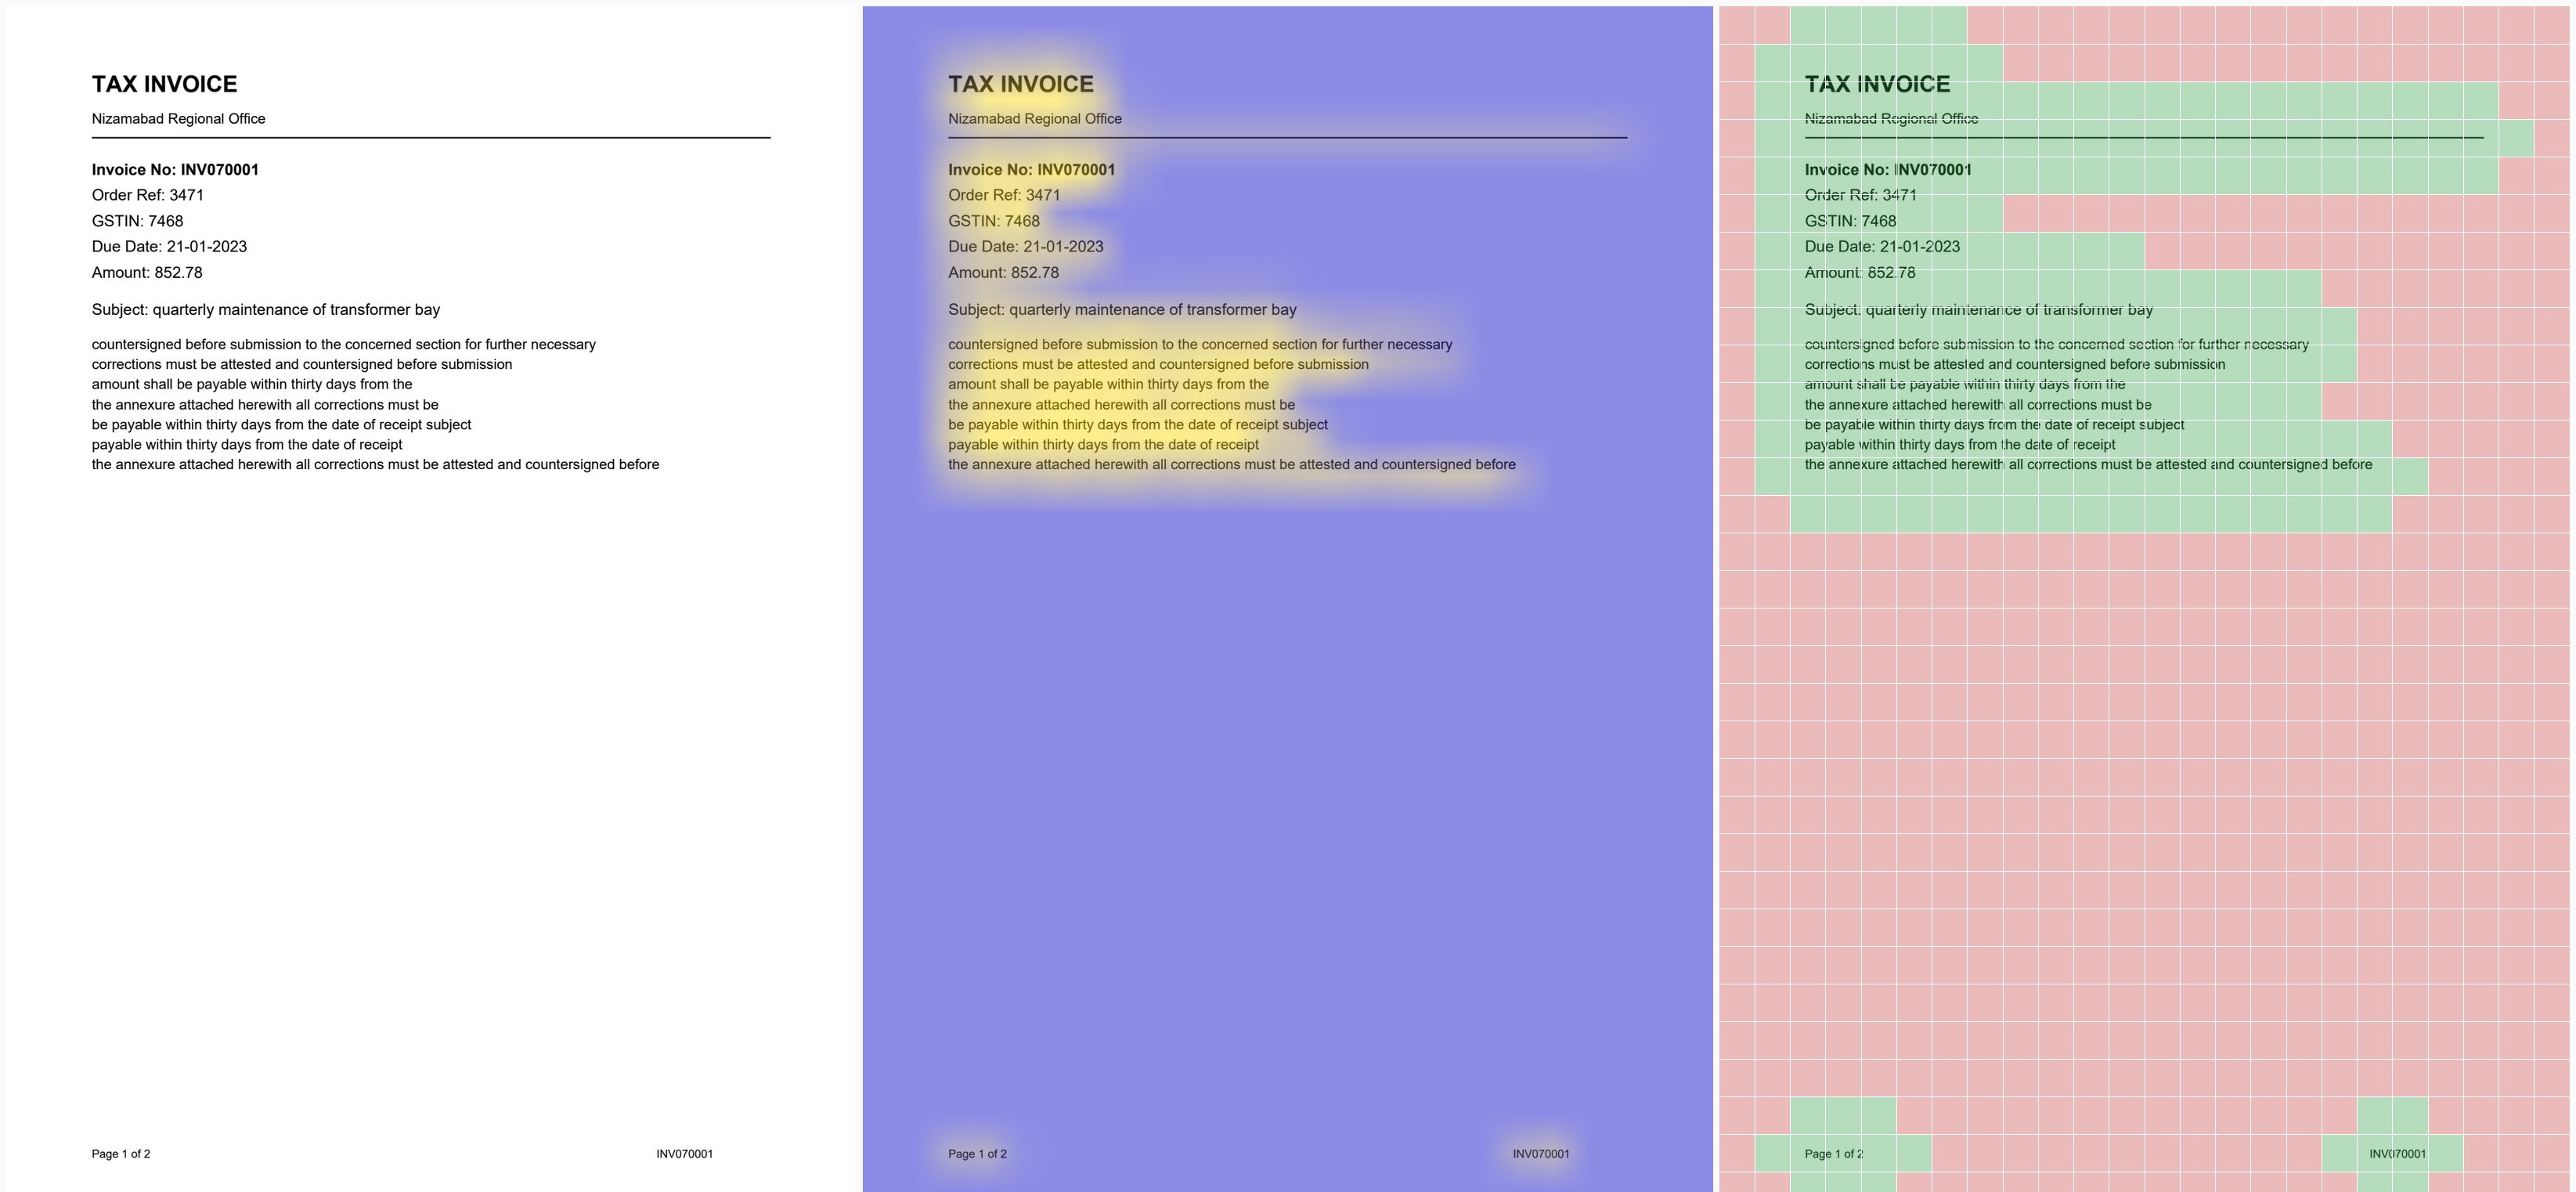
\includegraphics[width=\columnwidth]{figs/pruning_example.png}
\caption{Spatial pruning on a page from the evaluation corpus. Left: the
rendered page. Centre: the pixel-space saliency map. Right: the retained patch
mask, green for kept and red for discarded --- $233$ of $768$ grid patches
($30\%$) survive, and after redundancy collapsing $233$ of $875$ vectors
($27\%$) are stored. The retained region tracks the text block, and the margins,
which occupy most of the page, cost nothing.}
\label{fig:pruning}
\end{figure}

\subsection{Stage 2: embedding-space redundancy pruning}
Stage 1 removes patches with \emph{no} content. Stage 2 removes patches with
\emph{duplicate} content: the interior of a filled table cell, the middle of a
thick rule, a run of uniform texture inside a photograph. These are salient to a
pixel detector and yet contribute nothing to a MaxSim score. We visit the
survivors in descending saliency order and greedily form clusters of vectors
within cosine $\theta = 0.92$ of the representative, replacing each cluster with
its renormalised mean.

This is close to free in ranking terms for a structural reason. MaxSim takes, per
query vector, the maximum similarity over document vectors. If two document
vectors lie within cosine $\theta$ of one another, the maximum over the pair and
the similarity to their renormalised mean differ by an amount bounded by their
angular spread, which is small by construction --- so collapsing a tight cluster
barely moves the score while removing one stored vector per duplicate. The
argument does not extend to loose clusters, which is why $\theta$ is set high.

\subsection{Stage 3: quantization and asymmetric scoring}
A 128-dimensional float32 vector occupies $512$ bytes; retaining only the sign of
each dimension gives $128$ bits, or $16$ bytes --- a flat $32\times$ on everything
the pruner allowed through. These vectors are L2-normalised with approximately
zero-centred dimensions, so $\mathrm{sign}(\mathbf{d})$ preserves the orthant of
$\mathbf{d}$ and discards only its position within that orthant.

We score asymmetrically: the document side is binarised, the query side is not.
A fully symmetric scheme reduces MaxSim to a popcount Hamming distance and is
cheaper still, but it discards the query magnitudes --- and those are precisely the
part that can be afforded, since a query contributes on the order of twenty
vectors against a corpus of millions. Asymmetric scoring costs one unpack and one
float matrix product and recovers most of the ranking quality; the symmetric
variant is retained only for comparison. For a query matrix $Q$ and a page's code
matrix $C$,

\begin{equation}
\mathrm{MaxSim}(Q, C) = \sum_{i} \max_{j} \; \mathbf{q}_i \cdot \mathrm{sign}(\mathbf{d}_j).
\end{equation}

We also evaluate an int8 codec at $4\times$. Because the components of an
L2-normalised $128$-dimensional vector concentrate near $1/\sqrt{d}$ --- the
observed mean absolute component is $0.071$ and the observed maximum $0.363$ ---
the textbook $\mathrm{round}(127v)$ mapping, which assumes the data spans
$[-1,1]$, leaves roughly two thirds of the available levels permanently unused.
Rescaling by the range the data actually occupies costs no additional storage and
reduces the mean cosine error on real vectors from $3.28 \times 10^{-4}$ to
$8.20 \times 10^{-5}$.

\subsection{Memory accounting}
\label{sec:memory}
One implementation detail is load-bearing for the claims in this paper. A naive
scorer decodes the packed index into a float32 matrix before computing
similarities, which restores the full $d \times 4$ bytes per vector at query time
and returns the entire saving --- an index of $2.82$~KB per page on disk demanded
$90.12$~KB per page in RAM to search. The storage claim was true while the
system-level claim behind it was not. We therefore score in blocks sized against
a memory budget, releasing each block before the next is allocated; peak resident
memory then tracks the budget (measured at $0.93\times$ of it) and is independent
of corpus size, while producing scores bit-identical to the cached path.
All index sizes reported below are computed from the pipeline's own byte
accounting rather than from files on disk, so they are neither inflated by
container overhead nor deflated by filesystem compression.

\section{Experimental Setup}

\subsection{Configuration}
Three experiments share one pipeline, one measurement protocol and one code
path, differing only in encoder and corpus. We label them E1, E2 and E3
throughout. E1 and E2 differ in both variables at once; E3 exists to separate
them, and forms the fourth cell of a $2 \times 2$ over $\{$small,
reference$\}$ encoders and $\{$generated, real$\}$ pages.

\emph{E1: small encoder, generated corpus.} The encoder is
\texttt{vidore/colSmol-256M} (ColIdefics3), float32, on CPU; hardware is a laptop
with $8$~GB of DDR4 and no GPU. The corpus is $60$ generated pages ($30$ documents
of $2$ pages) rendered at A4, $150$~dpi. The encoder emits $875$ vectors per page
before compression ($768$ page-grid patches, $64$ thumbnail, $43$ instruction).

\emph{E2: reference encoder, ViDoRe.} The encoder is ColPali-v1.3 ($3$B
parameters) in bfloat16 on a single Tesla T4. The corpus is four ViDoRe test
splits --- \texttt{docvqa} ($500$ pages, $451$ queries), \texttt{syntheticDocQA
energy} ($500$, $100$), \texttt{infovqa} ($500$, $494$) and \texttt{tabfquad}
($280$, $280$) --- for $1{,}780$ pages and $1{,}325$ queries in total, with the
benchmark's own ground truth. The encoder emits $1{,}031$ vectors per page.

\emph{E3: reference encoder, generated corpus.} ColPali-v1.3 as in E2, over
E1's corpus. The generator is deterministic, so regenerating at seed $7$
reproduces the pages E1 measured rather than pages resembling them; we verified
that the manifests match. The encoder emits $1{,}031$ vectors per page, as in
E2. E1 and E3 therefore share a corpus, E2 and E3 share an encoder, and each
comparison isolates one variable.

Vector dimension is $128$ in all three and every run uses seed $1337$.

One implementation detail is worth recording, because it silently produces
plausible numbers. ColPali is published as a LoRA adapter over a PaliGemma base.
On current \texttt{transformers} and PEFT releases the adapter's key prefixes do
not match the names of the injected modules, so the projection head is created and
then left randomly initialised; the loader reports it as a missing key rather than
as an error. A benchmark run in that state completes normally and yields a
complete, well-formed, meaningless table. We therefore load the merged-weight
checkpoint, which contains no adapter to mis-key, and our loader refuses to run if
any parameter remains unmaterialised after loading.

\subsection{Queries and ground truth}
E1 has $72$ queries in two deliberately different families. Sixty
\emph{precise} queries pair a subject with a unique identifier and have exactly
one relevant page; these check that compression has not broken retrieval
outright. Twelve \emph{topical} queries name only a subject shared by several
pages, so the metric depends on \emph{ordering} a group of near-identical
candidates --- which is where compression damage becomes visible. Ground truth is
exact by construction.

E2 uses the queries and relevance judgements shipped with each ViDoRe split, so
the query distribution is the benchmark's rather than ours. The precise/topical
distinction is a property of our generator and does not carry over, so E2 is
reported per split instead.

\subsection{Controls}
Two choices make the ablation a controlled experiment rather than a leaderboard.

\emph{Exact scoring.} Every quality figure comes from exhaustive brute-force
MaxSim, not from an approximate index. An ANN structure would contribute its own
recall loss and confound the attribution we are trying to make. The Qdrant
backend is tested separately and is the deployment path, not the measurement
path.

\emph{One encoding pass.} The corpus is encoded once into a cache and every
ablation row replays over those identical vectors. Nothing but the compression
setting differs between rows, so a difference in a metric can have no other
cause. Re-running the benchmark reproduces the reported figures exactly; the
pipeline is deterministic given a fixed corpus and encoder.

\subsection{Metrics}
We report nDCG@5 with binary relevance (the standard ViDoRe metric), Recall@1 and
Hit@5, index bytes per page, and the compression ratio against the uncompressed
float32 index. We additionally report \emph{retention} --- nDCG@5 as a fraction of
the baseline row --- and Kendall $\tau$-b against the \emph{baseline's own
ranking}. The last is the load-bearing metric here. Absolute quality answers
``is this retriever any good?'', which depends mostly on the choice of encoder;
$\tau$ answers ``did compression change the retriever's mind?'', which is the
only question this layer controls.

\section{Results}

\begin{table*}[t]
\caption{\textbf{E1.} Ablation over the compression pipeline. $60$ pages,
$72$ queries, ColSmol-256M, exact MaxSim. Rows share one encoding pass, so every difference is
attributable to the compression setting alone. \emph{Retain} is nDCG@5 relative
to the baseline row; $\tau$ is Kendall $\tau$-b against the baseline's own
ranking.}
\label{tab:ablation}
\centering
\setlength{\tabcolsep}{4.5pt}
\resizebox{\textwidth}{!}{%
\begin{tabular}{@{}llrrrrrrrr@{}}
\toprule
\textbf{Variant} & \textbf{What it isolates} & \textbf{Tok/pg} & \textbf{KB/pg} &
\textbf{Compr.} & \textbf{nDCG@5} & \textbf{R@1} & \textbf{Hit@5} &
\textbf{Retain} & \textbf{$\tau$} \\
\midrule
baseline-float32 & reference: every patch, full precision & 875.0 & 448.00 & $1.0\times$ & 0.7823 & 0.5694 & 0.9722 & 100.0\% & 1.000 \\
\midrule
\multicolumn{10}{l}{\textit{Pruning alone (no quantization)}} \\
spatial-only & blank-patch pruning & 356.1 & 182.32 & $2.5\times$ & 0.7602 & 0.5694 & 0.9444 & 97.2\% & 0.935 \\
spatial+redundancy & both pruning stages & 246.8 & 126.34 & $3.5\times$ & 0.7519 & 0.5139 & 0.9722 & 96.1\% & 0.866 \\
\midrule
\multicolumn{10}{l}{\textit{Quantization alone (no pruning)}} \\
int8-only & scalar quantization & 875.0 & 112.00 & $4.0\times$ & 0.7877 & 0.5694 & 0.9861 & 100.7\% & 0.972 \\
binary-only & one-bit quantization & 875.0 & 14.00 & $32.0\times$ & 0.6875 & 0.4167 & 0.9444 & 87.9\% & 0.585 \\
\midrule
\multicolumn{10}{l}{\textit{Both stages}} \\
prune+int8 & quality-first operating point & 246.8 & 31.59 & $14.2\times$ & 0.7511 & 0.5139 & 0.9722 & 96.0\% & 0.864 \\
optivision & size-first operating point & 246.8 & 3.95 & $113.5\times$ & 0.6782 & 0.4028 & 0.9583 & 86.7\% & 0.606 \\
optivision-aggressive & fixed $25\%$ token budget & 186.3 & 2.98 & $150.3\times$ & 0.6680 & 0.3611 & 0.9722 & 85.4\% & 0.602 \\
\midrule
\multicolumn{10}{l}{\textit{Token-budget sweep, all with one-bit codes}} \\
keep-50\% & top $50\%$ by saliency & 288.1 & 4.61 & $97.2\times$ & 0.6704 & 0.4167 & 0.9444 & 85.7\% & 0.548 \\
keep-40\% & top $40\%$ by saliency & 263.6 & 4.22 & $106.2\times$ & 0.6721 & 0.4167 & 0.9583 & 85.9\% & 0.561 \\
keep-30\% & top $30\%$ by saliency & 241.6 & 3.87 & $115.9\times$ & 0.6721 & 0.4028 & 0.9583 & 85.9\% & 0.588 \\
keep-20\% & top $20\%$ by saliency & 206.1 & 3.30 & $135.9\times$ & 0.6676 & 0.3750 & 0.9722 & 85.3\% & 0.586 \\
keep-10\% & top $10\%$ by saliency & 162.9 & 2.61 & $171.8\times$ & 0.6700 & 0.4167 & 0.9306 & 85.6\% & 0.551 \\
\bottomrule
\end{tabular}}
\end{table*}

Table~\ref{tab:ablation} is the full E1 ablation and Fig.~\ref{fig:tradeoff}
plots it. Table~\ref{tab:colpali} is the same ablation under E2 on the split with
the most queries, and Table~\ref{tab:splits} gives retention across all four.
Three findings follow. Each is stated as E1 supports it and then tested against
E2, and only the first survives in the form E1 suggested.

\begin{figure}[t]
\centering
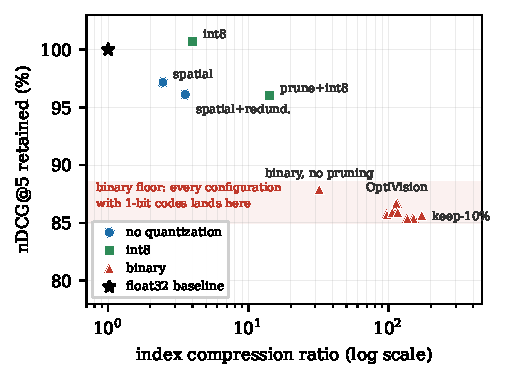
\includegraphics[width=\columnwidth]{figs/tradeoff.pdf}
\caption{\textbf{E1.} Compression ratio against nDCG@5 retention, by quantizer.
The points separate by \emph{codec}, not by token count: everything with one-bit
codes falls into the shaded band between $85\%$ and $88\%$ retention whether it
prunes nothing or prunes to a tenth, while the unquantized and int8
configurations stay above $96\%$. Fig.~\ref{fig:scale} shows what happens to this
picture under E2.}
\label{fig:tradeoff}
\end{figure}

\begin{table*}[t]
\caption{\textbf{E2.} The same ablation under ColPali-v1.3 on the ViDoRe
\texttt{docvqa} split ($500$ pages, $451$ queries), exact MaxSim, one encoding
pass shared by every row. Compare with Table~\ref{tab:ablation}: the binary rows
have moved from the mid-$80$s to the mid-$90$s, and the pruning rows have lost
most of their compression.}
\label{tab:colpali}
\centering
\setlength{\tabcolsep}{4.5pt}
\resizebox{\textwidth}{!}{%
\begin{tabular}{@{}llrrrrrrrr@{}}
\toprule
\textbf{Variant} & \textbf{What it isolates} & \textbf{Tok/pg} & \textbf{KB/pg} &
\textbf{Compr.} & \textbf{nDCG@5} & \textbf{R@1} & \textbf{Hit@5} &
\textbf{Retain} & \textbf{$\tau$} \\
\midrule
baseline-float32 & reference: every patch, full precision & 1031.0 & 527.87 & $1.0\times$ & 0.5841 & 0.4945 & 0.6608 & 100.0\% & 1.000 \\
\midrule
\multicolumn{10}{l}{\textit{Pruning alone (no quantization)}} \\
spatial-only & blank-patch pruning & 846.3 & 433.30 & $1.2\times$ & 0.5794 & 0.4945 & 0.6519 & 99.2\% & 0.873 \\
spatial+redundancy & both pruning stages & 557.5 & 285.43 & $1.8\times$ & 0.5691 & 0.4856 & 0.6386 & 97.4\% & 0.715 \\
\midrule
\multicolumn{10}{l}{\textit{Quantization alone (no pruning)}} \\
int8-only & scalar quantization & 1031.0 & 131.97 & $4.0\times$ & 0.5838 & 0.4989 & 0.6563 & 99.9\% & 0.919 \\
binary-only & one-bit quantization & 1031.0 & 16.50 & $32.0\times$ & 0.5625 & 0.4789 & 0.6364 & 96.3\% & 0.527 \\
\midrule
\multicolumn{10}{l}{\textit{Both stages}} \\
prune+int8 & quality-first operating point & 557.5 & 71.36 & $7.4\times$ & 0.5690 & 0.4878 & 0.6386 & 97.4\% & 0.712 \\
optivision & size-first operating point & 557.5 & 8.92 & $59.2\times$ & 0.5523 & 0.4545 & 0.6341 & 94.6\% & 0.510 \\
optivision-aggressive & fixed $25\%$ token budget & 156.1 & 2.50 & $211.3\times$ & 0.4874 & 0.4080 & 0.5610 & 83.4\% & 0.409 \\
\midrule
\multicolumn{10}{l}{\textit{Token-budget sweep, all with one-bit codes}} \\
keep-50\% & top $50\%$ by saliency & 373.9 & 5.98 & $88.2\times$ & 0.5404 & 0.4612 & 0.6142 & 92.5\% & 0.486 \\
keep-40\% & top $40\%$ by saliency & 309.0 & 4.94 & $106.8\times$ & 0.5276 & 0.4501 & 0.5987 & 90.3\% & 0.459 \\
keep-30\% & top $30\%$ by saliency & 239.8 & 3.84 & $137.6\times$ & 0.5076 & 0.4146 & 0.5942 & 86.9\% & 0.455 \\
keep-20\% & top $20\%$ by saliency & 165.3 & 2.64 & $199.6\times$ & 0.4778 & 0.3925 & 0.5543 & 81.8\% & 0.398 \\
keep-10\% & top $10\%$ by saliency & 86.0 & 1.38 & $383.6\times$ & 0.3899 & 0.3126 & 0.4634 & 66.7\% & 0.393 \\
\bottomrule
\end{tabular}}
\end{table*}

\begin{table}[t]
\caption{\textbf{E2.} nDCG@5 retained across all four ViDoRe splits. The
\texttt{energy} split has only $100$ queries and reads above $100\%$ for most
rows; those differences are noise, not improvement. Compression ratios are
rounded to whole numbers above $50\times$.}
\label{tab:splits}
\centering
\setlength{\tabcolsep}{2.4pt}
\begin{tabular}{@{}lrrrrr@{}}
\toprule
\textbf{Variant} & \textbf{docvqa} & \textbf{energy} & \textbf{infovqa} &
\textbf{tabfquad} & \textbf{Compr.} \\
\midrule
spatial-only & 99.2\% & 101.1\% & 99.8\% & 99.8\% & $1.0$--$1.4\times$ \\
spatial+redundancy & 97.4\% & 101.8\% & 99.7\% & 99.2\% & $1.7$--$1.9\times$ \\
int8-only & 99.9\% & 101.6\% & 100.1\% & 99.9\% & $4.0\times$ \\
binary-only & 96.3\% & 100.6\% & 97.4\% & 100.3\% & $32.0\times$ \\
prune+int8 & 97.4\% & 101.6\% & 99.5\% & 99.8\% & $6.7$--$7.5\times$ \\
optivision & 94.6\% & 103.4\% & 97.2\% & 95.6\% & $53$--$60\times$ \\
keep-50\% & 92.5\% & 101.8\% & 94.7\% & 97.4\% & $81$--$91\times$ \\
keep-10\% & 66.7\% & 89.8\% & 85.4\% & 81.6\% & $342$--$387\times$ \\
\bottomrule
\end{tabular}
\end{table}

\subsection{Finding 1: pruning is close to free, and buys less than it appears}
Under E1, removing blank patches costs $2.8\%$ of nDCG@5 for a $2.5\times$ token
reduction, and adding redundancy collapsing brings this to $3.5\times$ for
$3.9\%$. Rank agreement with the uncompressed baseline remains high throughout
($\tau = 0.87$--$0.94$), and \texttt{spatial-only} matches the baseline exactly on
Recall@1 ($0.5694$): discarding $59\%$ of the vectors does not cost a single top-1
hit.

Under E2 the quality claim holds more strongly and matters much less. Both
pruning stages together retain $97.4$--$101.8\%$ of nDCG@5 across the four splits,
but the token reduction collapses from $3.5\times$ to $1.7$--$1.9\times$. The
reason is visible in the extreme case: on \texttt{infovqa}, spatial pruning keeps
$1{,}000$ of $1{,}031$ patches and saves essentially nothing. Wide margins are a
property of the documents our generator renders, not of documents in general, and
ViDoRe --- scans, infographics, dense tables --- does not have them. The claim
survives; the number behind it does not.

\subsection{Finding 2: the token budget is free only when the corpus is sparse}
\label{sec:sweep}
Under E1 the token-budget sweep is almost flat. Keeping the
top $10\%$ of patches --- $163$ vectors per page --- retains $85.6\%$ of nDCG@5,
while keeping the top $50\%$ --- $288$ vectors, a $1.8\times$ larger index ---
retains $85.7\%$. The $0.1$ point separating them is well inside the noise of $72$
queries, which invites the conclusion that the token budget is not the operative
variable once a codec is fixed.

Under E2 that conclusion fails outright. Keeping the top $10\%$ retains $66.7\%$
on \texttt{docvqa}, $81.6\%$ on \texttt{tabfquad} and $85.4\%$ on
\texttt{infovqa}, against $92.5\%$, $97.4\%$ and $94.7\%$ at the top $50\%$
(Table~\ref{tab:splits}). The flat sweep was an artifact of a corpus whose salient
content fits comfortably inside the top $10\%$ of patches; on pages where it does
not, the aggressive setting is a genuine trade rather than a free $1.8\times$.

\subsection{Finding 3: the one-bit penalty follows the decision margin, not the encoder}
\label{sec:finding3}
Under E1, \texttt{binary-only} loses $12.1\%$ of nDCG@5 \emph{without discarding a
single token}, and its $\tau$ of $0.585$ says it substantially reorders results
rather than merely rescaling scores. Against this, \texttt{int8-only} costs
nothing measurable at $4\times$ --- $100.7\%$ retention with $\tau = 0.972$, the
excess above $100\%$ being noise at $72$ queries. Every E1 configuration that includes
one-bit codes lands in a narrow $85$--$88\%$ retention band regardless of how much
pruning is applied. Under E2 the band is gone: \texttt{binary-only} retains
$96.3\%$ on \texttt{docvqa} and $97.4\%$ on \texttt{infovqa}. Under E3 --- ColPali
over E1's own pages --- it retains $98.4\%$ with R@1 unchanged at $0.375$. A
$12.1\%$ penalty became $1.6\%$ under a change of encoder alone, with the codec
and the pages untouched (Table~\ref{tab:dissociation}).

The reading that suggests itself --- that the codec's cost is a property of the
encoder --- does not survive a per-query look at the same caches. For each query
we take the float-precision margin $m$ by which the gold page beats its best
non-relevant competitor, as a fraction of the gold score, and the noise $\sigma$
a codec adds to page scores, measured as the residual of the codec's scores
around a linear fit to the float scores in the same units. A sign code adds
$\sigma \approx 2.8\%$ of the score under ColSmol and $2.5\%$ under ColPali; a
two-bit code about half that; int8 $0.06\%$. The noise is a property of the
codec, and it is the same for both encoders. What differs is where the queries
sit. E1's $60$ \emph{precise} queries are decided by three digits inside a
nine-character code, and the retriever resolves them by a median margin of
$0.05\%$ (interquartile $-0.7\%$ to $+0.9\%$): the gold page is effectively tied
with its same-subject neighbour before any codec is applied. The $12$ topical
queries are won by $31\%$. Under every codec, on every cache we hold (six
ColSmol, two ColPali), \emph{no query whose margin exceeds $2\sigma$ changes its
top result}, while $32$--$43\%$ of those below $0.5\sigma$ do; among the queries
the float retriever wins, the margin alone separates the ones a sign code keeps
from the ones it loses with AUC $0.78$--$0.95$ (Table~\ref{tab:margin}).

\begin{table}[t]
\caption{Per-query decision margin against codec noise, both as a fraction of
the gold page's float score. $m$ is the median float margin of the $60$ precise
queries; $\sigma$ is the score noise a codec adds; flip rates are the share of
queries whose top-$1$ result changes under the sign code, by $|m|/\sigma$ bin;
AUC is how well $m$ alone separates the float winners the sign code keeps from
those it loses. Rows are the E1 encoder (ColSmol) and the E3 encoder (ColPali)
on the same $60$ pages with the code's glyphs at the stated size; the ColSmol
rows re-render only those glyphs, the ColPali $3\times$ row was rendered with the
code in the text flow, which also shifts the lines below it.}
\label{tab:margin}
\centering
\footnotesize
\setlength{\tabcolsep}{3pt}
\begin{tabular}{@{}lrrrrrr@{}}
\toprule
encoder, code & $m$ & $\sigma_{\mathrm{sign}}$ & $\sigma_{\mathrm{2bit}}$ & $<0.5\sigma$ & $>2\sigma$ & AUC \\
\midrule
ColSmol $1\times$ (E1) & $-0.05\%$ & $2.8\%$ & $1.5\%$ & $32\%$ & $0\%$ & $0.78$ \\
ColSmol $3\times$ & $-0.31\%$ & $2.7\%$ & $1.4\%$ & $32\%$ & $0\%$ & $0.90$ \\
ColSmol $0.4\times$ & $-0.65\%$ & $2.8\%$ & $1.6\%$ & $41\%$ & $0\%$ & $0.94$ \\
ColPali $1\times$ (E3) & $-1.39\%$ & $2.5\%$ & $1.3\%$ & $43\%$ & $0\%$ & $0.86$ \\
ColPali $3\times$ & $-0.52\%$ & $2.2\%$ & $1.2\%$ & $40\%$ & $0\%$ & $0.88$ \\
\bottomrule
\end{tabular}
\end{table}

This is also why ColPali appears immune. On E1's pages it wins $15$ of the $60$
precise queries in float, three more than the $12$ a subject-only ranker gets by
chance, and its median precise-query margin is $-1.4\%$: it cannot read an
$11$\,pt code at $448$\,px and has lost those queries before any quantization.
Under the sign code seven of them flip from won to lost and seven from lost to
won, which nets to the ``unchanged'' R@1 of $0.375$. Re-rendering only the
code's glyphs three times larger, with every other line, the generator's random
sequence and the queries held fixed, lifts ColPali's precise R@1 to $0.317$ and
its one-bit cost from $1.6\%$ to $4.1\%$, with precise R@1 under the sign code
back at $0.233$: the encoder starts winning near-tie queries and starts losing
them to the codec. At $72$ queries the aggregate change is inside the noise
(paired over identical queries, $-0.019$ nDCG@5, $95\%$ CI $[-0.094, +0.058]$),
so we report it as a direction; the per-query structure in
Table~\ref{tab:margin} is the measurement. The same manipulation on ColSmol, at
$0.4\times$, $1\times$ and $3\times$ the code size, moves the float retriever
(precise R@1 $0.283$, $0.483$, $0.333$ --- a $33$\,pt code spans three patches,
and no single document vector then holds the string a query vector must match)
but leaves the one-bit cost at $9.6\%$, $12.1\%$ and $9.0\%$, with paired
differences of $+0.03$ nDCG@5 and intervals through zero. Glyph size, like
encoder identity, is not the variable.

The statement that survives is narrower than the one the aggregate numbers
invite, and more useful: \emph{a codec costs the queries whose decision margin is
smaller than its score noise.} E1 is the worst case by construction --- $40$ of
its $72$ queries sit below $0.5\sigma$ for a sign code --- E3 is a floor, and E2's
$2.6$--$3.7\%$ measures how many ViDoRe queries are within about $3\%$ of a tie.
Pruning's yield, by contrast, does answer to the corpus and only to the corpus:
$4.2\times$ to $1.9\times$ under one encoder, $3.6\times$ to $4.2\times$ under
one corpus. At reference scale neither stage binds: compression to roughly
$57\times$ is nearly free, and the limit on the pipeline is how little a
pixel-space saliency detector can remove from a dense page.

\begin{figure}[t]
\centering
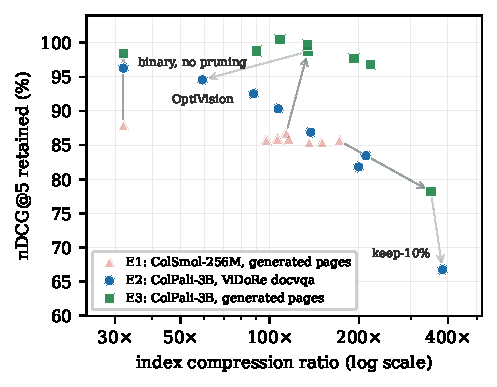
\includegraphics[width=\columnwidth]{figs/scale.pdf}
\caption{The dissociation. Every configuration using one-bit codes, under all
three experiments, at the same compression ratios. Under E1 (red) they sit in a
band below $88\%$ retention; under E2 (blue) the same configurations retain
$94$--$97\%$. E3 (green) shares E1's pages and E2's encoder, and sits at or above E2,
clear of E1's band. Finding~3 shows why this is not an encoder property: E1's
band is made of near-tie queries that ColPali does not win in float precision
either. Dark arrows join identical configurations from E1 to E3, which changes
only the encoder; light arrows continue to E2, which changes only the corpus.}
\label{fig:scale}
\end{figure}

\begin{table}[t]
\caption{Each quantity against its own control. E3 shares E1's corpus and E2's
encoder, so the first four rows change exactly one thing; the last two change
nothing but the size of the one discriminative string on the page. Pruning's
yield answers to the corpus. The codec's cost moves with the encoder and moves
again with glyph size alone, and Finding~3 traces both to the queries' decision
margins. E2 figures are the \texttt{docvqa} split; the last two rows are at $72$
queries and inside their confidence intervals.}
\label{tab:dissociation}
\centering
\setlength{\tabcolsep}{3pt}
\begin{tabular}{@{}llr@{}}
\toprule
Quantity & Control & Change \\
\midrule
one-bit codec cost & corpus fixed, encoder swapped & $12.1 \to 1.6$ pts \\
one-bit codec cost & encoder fixed, corpus swapped & $1.6 \to 3.7$ pts \\
pruning yield & corpus fixed, encoder swapped & $3.6 \to 4.2\times$ \\
pruning yield & encoder fixed, corpus swapped & $4.2 \to 1.9\times$ \\
one-bit codec cost & ColPali, glyphs $3\times$ & $1.6 \to 4.1$ pts \\
one-bit codec cost & ColSmol, glyphs $0.4\times$/$3\times$ & $12.1 \to 9.6$/$9.0$ \\
\bottomrule
\end{tabular}
\end{table}

\subsection{Finding 4: on dense pages, coverage beats ink and nothing beats random}
\label{sec:selection}
Finding 2 leaves a question the pixel detector cannot answer: when the page is
dense and a token budget is imposed anyway, which tokens should go? The natural
alternative to ranking patches by ink is to rank them by how much of the
embedding space they cover --- score every document vector against a set of
probe directions and keep the ones that win a MaxSim most often, so that
whatever a query turns out to ask, some retained vector is near it. We built
this selector with $256$ probes chosen by greedy farthest-point traversal of a
$20{,}000$-patch sample of the corpus, and ran it on \texttt{infovqa} and
\texttt{docvqa} at three budgets against the two controls any such selector has
to beat: the same procedure with $256$ uniformly random unit vectors that have
never seen the corpus, and the pixel detector at the same budget
(Table~\ref{tab:selection}). Budgets match to within $3\%$ of tokens per page,
and every row uses the one-bit codec.

\begin{table}[t]
\caption{Token selection on dense pages: retention of float nDCG@5 at three
budgets, all rows one-bit. \texttt{pixel} is the saliency detector of Stage~1;
\texttt{coverage} keeps the patches that win most MaxSims against $256$
farthest-point probes; \texttt{random} is the same procedure with $256$ random
unit vectors. Budgets match to within $3\%$ of tokens per page; $494$ queries on
\texttt{infovqa}, $451$ on \texttt{docvqa}.}
\label{tab:selection}
\centering
\footnotesize
\setlength{\tabcolsep}{4pt}
\begin{tabular}{@{}llrrr@{}}
\toprule
split & budget & pixel & coverage & random \\
\midrule
\texttt{infovqa} & $50\%$ & $94.7\%$ & $96.2\%$ & $96.7\%$ \\
 & $30\%$ & $92.3\%$ & $95.9\%$ & $95.7\%$ \\
 & $10\%$ & $85.4\%$ & $89.6\%$ & $90.7\%$ \\
\texttt{docvqa} & $50\%$ & $92.5\%$ & $91.4\%$ & $92.3\%$ \\
 & $30\%$ & $86.9\%$ & $88.2\%$ & $90.5\%$ \\
 & $10\%$ & $66.7\%$ & $77.9\%$ & $76.9\%$ \\
\bottomrule
\end{tabular}
\end{table}

Two things are true at once. Coverage-based selection beats pixel saliency
below a $50\%$ budget on both splits, by $4$ points at $10\%$ on
\texttt{infovqa} and $11$ on \texttt{docvqa}: on a dense page the ink ranking
discards the vectors queries actually match. And the probe construction
contributes nothing to that. Random probes are within one point of the designed
probes at every budget on \texttt{infovqa}, ahead by one to two points at
$50\%$ and $30\%$ on \texttt{docvqa}, and behind by one at $10\%$; across $945$
queries no selector we tried beats random. This reproduces, for a different
selector and a different encoder, the observation of Ma
et~al.~\cite{lightcolpali} that random pruning outperforms saliency-based
pruning for ColPali, and we read it as a statement about the corpus rather than
about any method. On these splits $74\%$ (\texttt{infovqa}) and $66\%$
(\texttt{docvqa}) of all patches win at least one MaxSim over the query set; the
set of winners fitted on half the queries covers $64\%$ and $52\%$ of the index
and retains $100\%$ and $99.7\%$ of nDCG@5 on the other half. That is the
ceiling for any query-agnostic selector on dense pages --- $1.6$--$1.9\times$ at
no loss --- and below it every selector falls off a cliff at a similar rate. A
learned selector for this regime has to beat uniformly random dropping at a
matched budget, and we would regard that as the minimum control for any future
claim of the kind.

\subsection{Two operating points}
\begin{table}[t]
\caption{The configurations that follow from each experiment. Under E1 the two
are a genuine exchange; under E2 and E3 the size-first point dominates on
nDCG@5, and only $\tau$ separates them. E3 is the most favourable point we
measure, but on sparse generated pages rather than real ones.}
\label{tab:operating}
\centering
\setlength{\tabcolsep}{4pt}
\begin{tabular}{@{}lllrl@{}}
\toprule
& \textbf{Goal} & \textbf{Configuration} & \textbf{Compr.} & \textbf{Retain} \\
\midrule
E1 & smallest index & prune + binary & $113.5\times$ & 86.7\% \\
E1 & quality per byte & prune + int8 & $14.2\times$ & 96.0\% \\
\midrule
E2 & smallest index & prune + binary & $53$--$60\times$ & 94.6--103.4\% \\
E2 & quality per byte & prune + int8 & $6.7$--$7.5\times$ & 97.4--101.6\% \\
\midrule
E3 & smallest index & prune + binary & $134.5\times$ & 98.7\% \\
E3 & quality per byte & prune + int8 & $16.8\times$ & 102.3\% \\
\bottomrule
\end{tabular}
\end{table}

Table~\ref{tab:operating} summarises the practical consequence, and it differs
between the two regimes. Under E1 the choice is a real exchange: prune + binary
buys an $8\times$ smaller index than prune + int8 and pays $9.3$ points of
retention for it, and which side is correct is a deployment question.

Under E2 that exchange collapses. Prune + binary gives roughly $8\times$ the
compression of prune + int8 at the same nDCG@5, so on the headline metric the
size-first configuration simply dominates. What still separates them is ordering:
Kendall $\tau$ is $0.71$--$0.90$ for prune + int8 against $0.51$--$0.70$ for
prune + binary. A pipeline whose output is a shortlist for a downstream reader should
take the binary configuration and the $57\times$; one that shows a ranked list
directly to a person should still take int8, and the justification is $\tau$
rather than nDCG@5. This is a narrower and more specific recommendation than E1
alone would have produced, and it is the opposite of the one E1 alone would have
produced.

E3 makes the same recommendation more emphatically --- $134.5\times$ at $98.7\%$
retention --- but it should not be read as the headline. It combines the
corpus with the most blank paper to discard with an encoder that never wins the
near-tie queries a one-bit code would cost it (Finding~3), which is the best
case rather than a representative one. Its role here is to identify which
variable supplies which part of the gain.

\subsection{Latency}
Query latency falls with the token count, since MaxSim cost is linear in stored
vectors: under E1 from $3.25$~ms at the float32 baseline to $0.70$~ms at
keep-$10\%$ on $60$ pages, and under E2 on the $500$-page \texttt{docvqa} split
from 55.9~ms to 23.5~ms for the full pipeline and 4.4~ms at keep-$10\%$. We
do not emphasise these figures: the exact index used for measurement is not the
structure a deployment would use, and query encoding dominates search entirely at
this scale --- $65.7$~ms under E1 and 72.8~ms under E2.

\section{Discussion}

\subsection{What the one-bit codec costs, and why}
\label{sec:floor}
For random unit vectors the expected cosine between $\mathbf{d}$ and
$\mathrm{sign}(\mathbf{d})/\sqrt{d}$ is $\sqrt{2/\pi} \approx 0.798$, and it is
tempting to read an encoder's departure from that figure as its susceptibility
to one-bit codes. We measured it on every cache we hold: $0.800$ for ColSmol,
and $0.800$, $0.800$, $0.799$ and $0.801$ for ColPali on four corpora, against
the random reference of $0.798$. The statistic is a per-vector property of any
roughly isotropic $128$-dimensional distribution and carries no information
about retrieval. The same is true of the share of per-query-vector $\arg\max$
identities that change under the sign code, which is $75$--$83\%$ on every
cache, including those where the ranking barely moves. Neither quantity can be
the mechanism, and we withdraw both from the argument.

What a codec does to a ranking is decided one query at a time by two numbers.
The first is the noise it adds to a page's score, $\sigma$, which for a sign
code is $2.2$--$2.8\%$ of the score across both encoders and all corpora, for
the two-bit code about half that, and for int8 $0.06\%$; it is set by the codec
and, weakly, by how anisotropic the encoder's vectors are on that corpus. The
second is the margin $m$ by which the query's gold page leads its best
competitor in float, which is set by the corpus and by what the retriever can
read. A query flips when $|m| \lesssim \sigma$. On the generated corpus the
precise queries are near-ties by construction, so a sign code flips
$32$--$43\%$ of those below $0.5\sigma$ and none above $2\sigma$, under either
encoder; ColPali escapes only because its margins on those queries are negative
to begin with. On ViDoRe a sign code costs $2.6$--$3.7\%$, which is the
fraction of real queries within about $3\%$ of a tie, and it changes the
top-ranked page of $11\%$ of \texttt{infovqa} queries while nDCG@5 reports
$97.4\%$ retention --- a reason to report top-$1$ agreement alongside $\tau$.

The ladder of codecs follows. Int8 is lossless at $4\times$ on every cache
($99.9$--$100.2\%$). A rotated two-bit Lloyd--Max code at $16\times$ halves
$\sigma$ and recovers about half the sign code's loss everywhere ($99.4\%$ on
\texttt{infovqa}, $97.0\%$ on \texttt{docvqa}, $99.4\%$ on E3). The zero-byte
refinements of the sign code --- subtracting a global mean, an ITQ rotation, or
a ColBERTv2-style centroid with a one-bit residual~\cite{colbertv2} --- recover
$3$--$10$ points on E1, where $80\%$ of every page is blank paper and the mean
vector is the paper's direction, and nothing on ViDoRe: $+0.7$ ($95\%$ CI
$[-0.2, +1.8]$) and $+0.7$ $[-0.6, +2.0]$ on \texttt{infovqa} for centring and
ITQ, $-0.8$ $[-2.3, +0.7]$ and $-0.2$ $[-2.0, +1.6]$ on \texttt{docvqa}, and
$-4.2$ $[-6.5, -2.1]$ for the residual code on \texttt{docvqa} with its codebook
capped at $4{,}096$ centroids for $515{,}500$ vectors. The anisotropy those
refinements correct is a property of blank pages, not of the encoder, and it is
why E1 overstates their value.

\subsection{Implications}
Three follow. First, and most strongly, \emph{a reported compression ratio for
multi-vector retrieval should carry both a per-stage attribution and the encoder
and corpus it was measured on}. Our first two experiments differ only in those two
variables and produce opposite attributions from the same code; a paper reporting
either one alone would have supported a confident and wrong generalisation, and
it took a third run to establish which variable was responsible for which half
of the difference.

Second, the token budget is a free parameter exactly when the corpus is sparse,
and not otherwise. E1 would have licensed pruning as aggressively as the detector
allows; on ViDoRe that costs $25.8$ points of retention between the top $50\%$
and the top $10\%$. Sparsity is cheap to measure --- it is the fraction of
patches the saliency detector rejects --- and should be reported alongside any
token-reduction result.

Third, the research direction the attribution recommends is different in each
regime, which is the practical point of making the attribution at all. Where
queries are near-ties --- exact identifiers, codes, serial numbers on otherwise
similar pages --- the codec binds, the sign code is the wrong choice, and a
two-bit code at $16\times$ or int8 at $4\times$ is what a deployment should pay
for. Where queries are decided by wide margins the codec is nearly free and the
binding limit is the selector: on dense pages pixel saliency discards the
vectors queries match, coverage-based selection does better below a $50\%$
budget, and uniformly random probes do as well as any selector we tried
(Finding~4). A learned selector for this regime has to beat random at a matched
budget before it has earned anything. Shortlist rescoring remains attractive in
both, since Hit@5 stays well above nDCG@5 throughout --- the relevant page is
usually retrieved and merely misordered.

\subsection{Limitations}
\label{sec:limits}
We state these plainly, as they bound the claims above.

\emph{Corpus scale.} E2 uses $500$-page subsets of each ViDoRe split rather than
the full splits, so absolute nDCG@5 is not comparable with published leaderboard
figures. Only the ratios between rows are the measurement here, and those are what
we claim; but a larger corpus makes retrieval harder, and the compression
penalties we report may be optimistic in absolute terms.

\emph{Statistical power.} E1 has $72$ queries and the \texttt{energy} split of E2
has $100$, at which several rows read above $100\%$ retention. Those readings are
noise and we decline to interpret them; the \texttt{docvqa} ($451$) and
\texttt{infovqa} ($494$) splits carry the E2 conclusions. Every E3 aggregate
difference is likewise at $72$ queries and inside $\pm 0.08$ nDCG@5; the
per-query margin structure of Table~\ref{tab:margin}, not the aggregates,
carries the E3 conclusion.

\emph{Two points, one family.} We measure a $256$M and a $3$B encoder, both
ColBERT-style vision--language retrievers. E3 separates encoder from corpus, but two
points still do not locate a crossing: we cannot say at what scale the
attribution changes, nor whether parameter count or embedding quality is the
operative variable. The decision-margin rule of Finding~3 is verified on the
generated corpus, eight caches deep, and is a prediction rather than a
measurement on ViDoRe, whose caches we did not retain. The ColPali run with the
enlarged code was rendered with the code in the text flow, which also shifts
the lines below it; the three ColSmol runs hold every other pixel fixed.

\emph{Generator realism.} On E3's pages ColPali-v1.3 scores \emph{below}
ColSmol-256M (nDCG@5 $0.6954$ against $0.7823$). A $3$B reference encoder losing
to a $256$M one is a fact about our generated pages rather than about the
encoders, and it bounds what E1 and E3 can be taken to represent. It does not
affect the comparisons we draw from them, which are within-encoder ratios.

\emph{What $\tau$ measures.} Our $\tau$ is Kendall $\tau_b$ over the shared ids
of two top-$10$ hit lists, not over the full ranking; the same E1 run scores
$0.643$ over all $60$ pages, and the value moves with the cutoff ($0.402$ at
top-$5$, $0.691$ at top-$20$). It should therefore be read with its cutoff
named, and $\tau$ values are comparable across experiments only when the
candidate pool is a comparable fraction of the corpus --- which holds for E1
against E3, both $60$ pages, and not for either against E2's $500$. Where one
number is wanted we now prefer top-$1$ agreement and top-$5$ overlap with the
float ranking, which are free of a cutoff and report what a user would see;
under the sign code on \texttt{infovqa} they are $0.89$ and $0.77$.

\emph{Scoring path.} All quality numbers come from exact brute-force MaxSim,
deliberately. A deployment on an approximate index would see additional recall
loss from the ANN structure, which our figures do not include and were designed
not to include.

\section{Conclusion}

We built a model-agnostic compression layer for vision--language document
retrieval and used it to ask which of its two stages the retrieval quality is
actually paid to. Asking the question twice is what the paper turns on. Under a
$256$M encoder on generated pages the two stages are sharply asymmetric: pruning
costs $3.9\%$ of nDCG@5 for a $3.5\times$ token reduction while one-bit
quantization costs $12.1\%$ having discarded no tokens at all, and every binary
configuration lands in the same $85$--$88\%$ band. Under ColPali-v1.3 on four
ViDoRe splits the same code produces the opposite attribution: one-bit
quantization costs at most $3.7\%$, the full pipeline reaches $53$--$60\times$ at
$94.6$--$103.4\%$ retention, and what fails instead is the premise that a page is
mostly blank paper --- pruning yields $1.7$--$1.9\times$ on real pages, and a
token-budget sweep that was flat becomes a $25.8$-point drop.

A third experiment holds the corpus fixed and swaps only the encoder, and a
per-query analysis of the caches separates what that reversal confounded. The
corpus governs what pruning buys ($4.2\times$ to $1.9\times$ under one encoder).
The codec's cost is not an encoder property: a sign code adds the same
$2$--$3\%$ of score noise under either encoder, and it costs exactly the queries
whose float margin over the best competitor is smaller than that --- none above
twice the noise on any of eight caches. The generated corpus decides its precise
queries at a median margin of $0.05\%$, which is why the small encoder looks
fragile; the reference encoder never wins those queries in the first place,
which is why it looks immune, and enlarging the code until it can lifts its
precise R@1 off the floor and its one-bit cost with it. On dense pages,
selecting tokens by embedding coverage beats pixel saliency below a $50\%$
budget and nothing beats uniformly random probes. The conclusion is therefore
not that the codec binds, nor that the token count binds, but that neither is a
property of the compression layer alone. A compression ratio for multi-vector
retrieval should be published with a per-stage attribution and with the
encoder, corpus and query regime that attribution was measured on, because the
attribution itself is what moves.

Future work follows directly: verify the decision-margin rule on the ViDoRe
caches, where it is so far a prediction; place the two-bit code, which halves
the sign code's noise at twice its bytes, at the operating point for near-tie
query regimes; hold any learned token selector to the random-dropping control
at a matched budget; and test shortlist rescoring, which our Hit@5 figures
suggest should recover most of the remaining ranking loss at negligible cost.

\section*{Acknowledgment}
The authors thank the Department of Emerging Technologies, Mahatma Gandhi
Institute of Technology, for supporting this work.

\begin{thebibliography}{00}

\bibitem{colpali}
M. Faysse, H. Sibille, T. Wu, B. Omrani, G. Viaud, C. Hudelot and P. Colombo,
``ColPali: Efficient Document Retrieval with Vision Language Models,''
in \emph{Proc. Int. Conf. on Learning Representations (ICLR)}, 2025.

\bibitem{colbert}
O. Khattab and M. Zaharia, ``ColBERT: Efficient and Effective Passage Search via
Contextualized Late Interaction over BERT,'' in \emph{Proc. 43rd Int. ACM SIGIR
Conf. on Research and Development in Information Retrieval}, 2020, pp. 39--48.

\bibitem{colbertv2}
K. Santhanam, O. Khattab, J. Saad-Falcon, C. Potts and M. Zaharia, ``ColBERTv2:
Effective and Efficient Retrieval via Lightweight Late Interaction,'' in
\emph{Proc. NAACL-HLT}, 2022, pp. 3715--3734.

\bibitem{pq}
H. J\'egou, M. Douze and C. Schmid, ``Product Quantization for Nearest Neighbor
Search,'' \emph{IEEE Trans. Pattern Anal. Mach. Intell.}, vol. 33, no. 1,
pp. 117--128, 2011.

\bibitem{binaryhash}
I. Yamada, A. Asai and H. Hajishirzi, ``Efficient Passage Retrieval with Hashing
for Open-domain Question Answering,'' in \emph{Proc. ACL-IJCNLP}, 2021,
pp. 979--986.

\bibitem{dynamicvit}
Y. Rao, W. Zhao, B. Liu, J. Lu, J. Zhou and C.-J. Hsieh, ``DynamicViT: Efficient
Vision Transformers with Dynamic Token Sparsification,'' in \emph{Advances in
Neural Information Processing Systems (NeurIPS)}, vol. 34, 2021,
pp. 13937--13949.

\bibitem{tome}
D. Bolya, C.-Y. Fu, X. Dai, P. Zhang, C. Feichtenhofer and J. Hoffman, ``Token
Merging: Your ViT But Faster,'' in \emph{Proc. Int. Conf. on Learning
Representations (ICLR)}, 2023.

\bibitem{hnsw}
Y. A. Malkov and D. A. Yashunin, ``Efficient and Robust Approximate Nearest
Neighbor Search Using Hierarchical Navigable Small World Graphs,'' \emph{IEEE
Trans. Pattern Anal. Mach. Intell.}, vol. 42, no. 4, pp. 824--836, 2020.

\bibitem{dse}
X. Ma, S.-C. Lin, M. Li, W. Chen and J. Lin, ``Unifying Multimodal Retrieval via
Document Screenshot Embedding,'' in \emph{Proc. EMNLP}, 2024, pp. 6600--6611.

\bibitem{lightcolpali}
Y. Ma, J. Li, Y. Zang, X. Wu, X. Dong, P. Zhang, Y. Cao, H. Duan, J. Wang,
Y. Cao and A. Sun, ``Towards Storage-Efficient Visual Document Retrieval: An
Empirical Study on Reducing Patch-Level Embeddings,'' in \emph{Findings of the
Association for Computational Linguistics: ACL 2025}, 2025. arXiv:2506.04997.

\bibitem{qdrant}
Qdrant, ``Multivectors, Binary Quantization and Rescoring,'' Qdrant
Documentation. [Online]. Available: \url{https://qdrant.tech/documentation/}

\end{thebibliography}

\end{document}
